\section{Model 1 Results}

Looking to results of the model i use the optimal $\beta_L = 3.43$ and simulate 5000 agents using Value Function Iteration Solution. Since all the solution methods yield the same results, I've arbitrarily choosen the VFI agent. Using the 5000 simulations I can find relevant summary statistics for infering wether or not the model fit the data and out assumptions about what is expected from the real world. Looking the  first plot of the simulated data set figure \ref{fig:dqi_model1_average_path_sim_vs_empirical} the empirical number of hours supplied by women \textbf{LIGEF15} compared to the simulated, where again only women actually in the labour force $H>0$ is considered. Looking to the fit of the data, the results are reasonable. In general the simulated data set slightly overestimates the number of supplied hours, especially around age 30, where the number of supplied hours are higher. The simulated data show heterogeneous variance over the life cycle, where especially the later stages of the life cycle show higher variance. This could very well stem from the idiosyncratic wage path increasing over time. Considering the estimation method where indirect inference is used using the number of supplied hours, it is not surprising that this is where the model performs the best. 


\begin{figure}
    \centering
    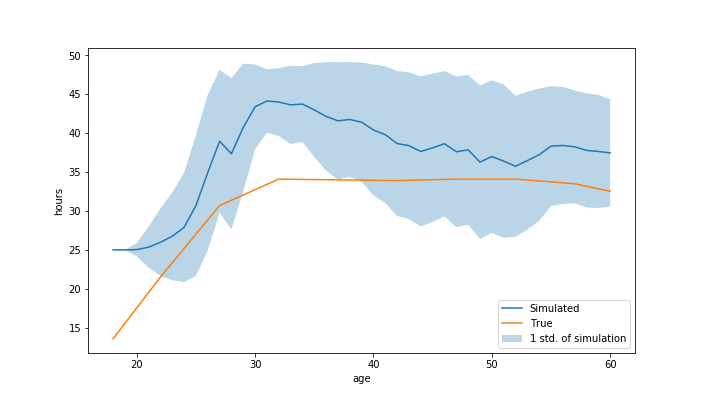
\includegraphics[scale=0.4]{figures/dqi_model1_estimation_labour_supply.png}
    \caption{Average Number of Supplied Working Hours - Empirical Vs. Simulated}
    \label{fig:dqi_model1_average_path_sim_vs_empirical}
\end{figure}

Figure \ref{fig:dqi_model1_fraction_in_workforce} shows the fraction of women in the workforce in the simulated data set. From here it is very clear, that the model underestimates the number of women working! From age 25, 80 \% of the women is out of the workforce, witch a slow decline in participation going forward to retirement. This is does obviously not correspond what can be observed in the real world. Even though it's not possible to get acces to exact number of women out of the labour force conditional on age, it can be approximated. Using \textbf{FOLK1B} supplied by Statistics Denmark the number of women in the age (15 to 60) can be found. Using that data the number of relevant women (considering the age) is around 1.664 million people. Looking at the number of women not working for relevant reasons the can be summarized to: women not working due to: \textit{working in the home}, \textit{Studying}, \textit{Other people outside the labour force}. These add up to: $15 + 161 + 66 = 242$ thousand people or $0.242$ million people. Using these numbers the number of women in the relevant age group outside the labour force can be approximated to be the number given in equation \ref{eq:women_outside_the_labour_force}

\begin{equation}
    \label{eq:women_outside_the_labour_force}
    \textbf{Women outside the labour force} = \frac{0.242}{1.664} = 0.145 = 14.5 \%
\end{equation}

The estimation of $\beta_L$ has not taken this meassure into account, which might be a first way to solve the problem.

\begin{figure}
    \centering
    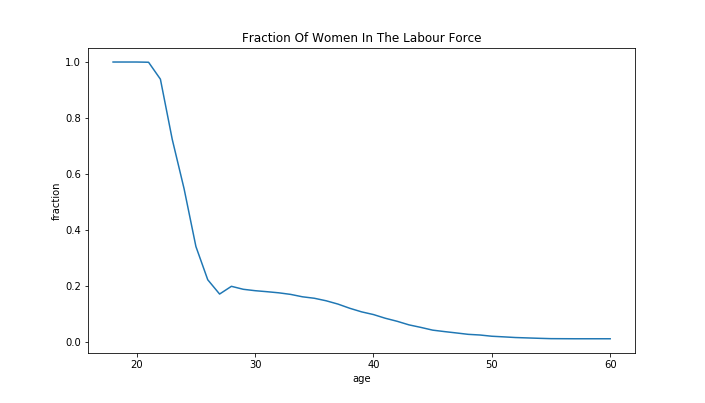
\includegraphics[scale=0.4]{figures/dqi_model1_women_in_labour_force_fraction.png}
    \caption{Fraction of Women in The Labour Force}
    \label{fig:dqi_model1_fraction_in_workforce}
\end{figure}

Both figure \ref{fig:dqi_model1_birth_onset} and figure \ref{fig:dqi_model1_child_vs_no_child_30} is inspired by the article \parencite{kleven_children_2019}. In the article the authors show how participation of women is affected when she gives birth to a child. In the paper they find that women  when giving birth to a child on average use 20 \% time less on work, immediately after the birth of the child, with a slow incremental return to normal ( with a long run penalty of aroun 6 \%. This is not the case in the simulations performed in these simulations. Getting a child, do seem to decrease the number of hours supplied however, the difference is indistinguishable from the mothers not getting children. This is clear in figure \ref{fig:dqi_model1_child_vs_no_child_30}, where first time mothers of age 30 is compared with women that have no children. The paths are indistinguishable, where the paper by \parencite{kleven_children_2019} would suggest a decrease of about 20 percent immediately after the birth (at age 31). These figures does not sort out women outside the labour force.


\begin{figure}
    \centering
    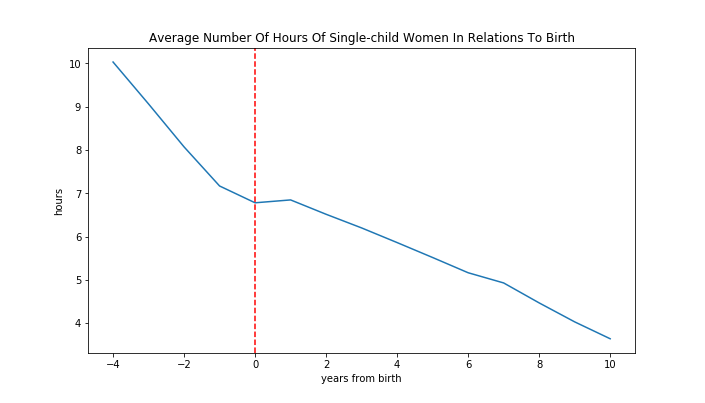
\includegraphics[scale=0.4]{figures/women_supplied_hours_dqi_model1_birth_onset.png}
    \caption{Average Number of Supplied hours, compared to birth onset.}
    \label{fig:dqi_model1_birth_onset}
\end{figure}


\begin{figure}
    \centering
    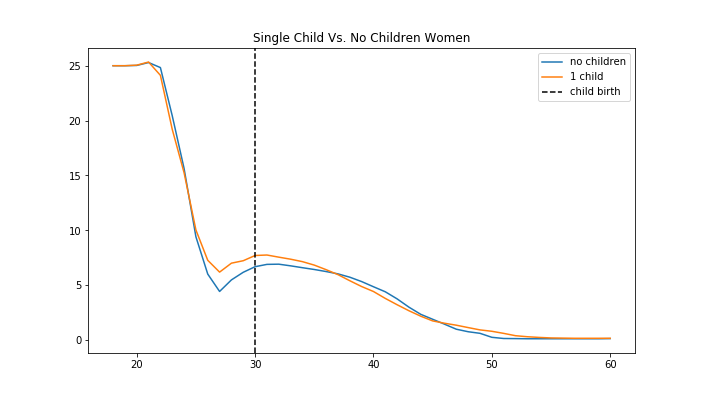
\includegraphics[scale=0.4]{figures/dqi_single_child_vs_no_child_model1.png}
    \caption{First time mothers (age 30) vs. Women with no children}
    \label{fig:dqi_model1_child_vs_no_child_30}
\end{figure}


